%%%%%%%%%%%%%%%%%%%%%%%%%%%%%%%%%%%%%%%%%%%%%%%%%%%%%%%%%%%%%%%%%%%%%%%%%%%%%%%%
%2345678901234567890123456789012345678901234567890123456789012345678901234567890
%        1         2         3         4         5         6         7         8

\documentclass[letterpaper, 10 pt, conference]{ieeeconf}  % Comment this line out if you need a4paper

%\documentclass[a4paper, 10pt, conference]{ieeeconf}      % Use this line for a4 paper

\IEEEoverridecommandlockouts                              % This command is only needed if 
                                                          % you want to use the \thanks command

\overrideIEEEmargins                                      % Needed to meet printer requirements.

%In case you encounter the following error:
%Error 1010 The PDF file may be corrupt (unable to open PDF file) OR
%Error 1000 An error occurred while parsing a contents stream. Unable to analyze the PDF file.
%This is a known problem with pdfLaTeX conversion filter. The file cannot be opened with acrobat reader
%Please use one of the alternatives below to circumvent this error by uncommenting one or the other
%\pdfobjcompresslevel=0
%\pdfminorversion=4

% See the \addtolength command later in the file to balance the column lengths
% on the last page of the document

% The following packages can be found on http:\\www.ctan.org
\usepackage{graphics} % for pdf, bitmapped graphics files
%\usepackage{epsfig} % for postscript graphics files
%\usepackage{mathptmx} % assumes new font selection scheme installed
%\usepackage{times} % assumes new font selection scheme installed
\usepackage{amsmath} % assumes amsmath package installed
\usepackage{amssymb}  % assumes amsmath package installed
\usepackage{xcolor}
\usepackage[hidelinks]{hyperref}
\usepackage{subcaption}
%\usepackage{graphicx}
\usepackage{wasysym}
\usepackage{ulem} 
\usepackage{tcolorbox}
\usepackage{booktabs} % for bottomrule, toprule, cmidrule
\usepackage{siunitx}
\usepackage{textcomp}

% my own style file
\usepackage{algorithm}
\usepackage[noend]{algpseudocode}
\usepackage{mathtools}	% the mathtools package loads \usepackage{amsmath}
\usepackage{amssymb}
\usepackage{siunitx}	% \SI{ #value }{ #unit }
\usepackage{cases}
\usepackage{color}
%\usepackage{graphicx}			<--- comment
\usepackage{xcolor}
\usepackage{lipsum}

\def\av{ \boldsymbol{a} }
\def\bv{ \boldsymbol{b} }
\def\mv{ \boldsymbol{m} }
\def\nv{ \boldsymbol{n} }
\def\pv{ \boldsymbol{p} }
\def\qv{ \boldsymbol{q} }
\def\sv{ \boldsymbol{s} }
\def\vv{ \boldsymbol{v} }
\def\xv{ \boldsymbol{x} }
\def\yv{ \boldsymbol{y} }
\def\Mm{ \boldsymbol{M} }
\def\Rm{ \boldsymbol{R} }
\def\Sm{ \boldsymbol{S} }
\def\Imat{ \boldsymbol{I} }
\def\omegav{ \omega }
\def\thetav{ \boldsymbol{\theta} }
\def\stage{\mathcal{S}}


\def\iunit{ \imath }	%similar to \imath and \jmath
\def\junit{ \jmath } %similar to \imath and \jmath (not available with the package mathptmx)
\def\kunit{ k } %similar to \imath and \jmath

\def\quaternion{	\xi 	}			%which is equal to \def\xiv{ \bldgreek{\xi} }
\def\qunit{ \xi				} 			%similar to \imath and \jmath
%\def\qr{	\xi 			}			%real number
\def\dq{	\check{\quaternion} 	}	% \boldsymbol #old: \boldmath{\check{\q}}
\def\dqunit{ \check{\xi}	} 			%similar to \imath and \jmath
\def\dual{	\varepsilon	}
\def\cconj{	^{*}			}			%complex conjugation
\def\dconj{	^{+}			}			%dual conjugation
\def\tconj{	^{\dagger}	}				%total conjugation

\def\quaternionnorm{ \operatorname{N}\!\left(\quaternion\right)	}	%quaternionic norm
\def\dqnorm{	\operatorname{N}\!\left(\dq\right)	}	%dual quaternionic norm

\def\pathpri{v}
\def\Pathpri{V\!}
\def\timepri{\zeta}

\newcommand{\sgn}[1]{ \operatorname{sgn}\! \left\{ #1 \right\} }%
%\newcommand{\qnorm}[1]{N\!\left(#1\right)}
%\newcommand{\qbetrag}[1]{\left|\left|#1\right|\right|_\ind{2}}

\definecolor{matlab1}{rgb}{0.0000, 0.4470, 0.7410}
\definecolor{matlab2}{rgb}{0.8500, 0.3250, 0.0980}
\definecolor{matlab3}{rgb}{0.9290, 0.6940, 0.1250}


\definecolor{matlab5}{rgb}{0.0000, 0.7059, 0.0000}
\definecolor{matlab7}{rgb}{0.7059, 0.0000, 0.0000}


%% Book Chapter -- Trajectory Generator
\def\SO3{ {SO\!\left(3\right)} }
%\def\SO2{ {SO\!\left(2\right)} }
\def\SE3{ {S\:\!\!E\!\left(3\right)} }
%\def\SE2{ {S\:\!\!E\!\left(2\right)} }
\def\E3{ {E\!\left(3\right)} }

\newcommand{\etal}{{et al.\;}}
\newcommand{\ie}{{i.e.\;}}			%id est = that is
\newcommand{\eg}{{e.g.\;}}
\newcommand{\wrt}{{w.r.t.\;}}		
\newcommand{\qed}{$\blacksquare$}

\newcommand{\timeprimitive}{\tau}
\newcommand{\pathprimitive}{s}

\newcommand{\vmax}{v_\text{max}}
\newcommand{\amax}{a_\text{max}}
\newcommand{\jmax}{j_\text{max}}

\newcolumntype{N}{>{\scriptsize}l}

\newcommand{\coordinateframe}[1]{\left\{#1\right\}}

\def\Ca{\textcolor{black}{C_{\mathrm{a}, n}}}
\newcommand{\Can}[1]{\textcolor{black}{C_{\mathrm{a}, #1}}}
\def\Cj{\textcolor{black}{C_{\mathrm{j}, n}}}
\newcommand{\Cjn}[1]{\textcolor{black}{C_{\mathrm{j}, #1}}}

\def\vlo{\textcolor{black}{v_\mathrm{lo}}}
\def\vcr{\textcolor{black}{v_\mathrm{cr}}}
\def\vsd{\textcolor{black}{v_\mathrm{sd}}}
\def\slo{\textcolor{black}{s_\mathrm{lo}}}
\def\scr{\textcolor{black}{s_\mathrm{cr}}}
\def\ssd{\textcolor{black}{s_\mathrm{sd}}}
\def\Tlo{\textcolor{black}{T_\mathrm{lo}}}
\def\Tcr{\textcolor{black}{T_\mathrm{cr}}}
\def\Tsd{\textcolor{black}{T_\mathrm{sd}}}
\def\Tble{\textcolor{black}{T_\mathrm{ble}}}
\def\Llo{\textcolor{black}{L_\mathrm{lo}}}
\def\Lcr{\textcolor{black}{L_\mathrm{cr}}}
\def\Lsd{\textcolor{black}{L_\mathrm{sd}}}
\def\motionlaw{\textcolor{black}{s}}

\def\vmax{\textcolor{black}{v_\mathrm{max}}}
\def\amax{\textcolor{black}{a_\mathrm{max}}}
\def\dmax{\textcolor{black}{d_\mathrm{max}}}

\def\pathpri{\textcolor{black}{v_{\mathrm{N},n}}}
\def\Pathpri{\textcolor{black}{V_{\mathrm{N},n}}}
\newcommand{\pathprin}[1]{\textcolor{black}{v_{\mathrm{N},#1}}}
\newcommand{\Pathprin}[1]{\textcolor{black}{V_{\mathrm{N},#1}}}
\def\timepri{\textcolor{black}{\tau}}

%% new
\def\C3{\textcolor{black}{\mathcal{C}^3}}
\def\Cn{\textcolor{black}{\mathcal{C}^n}}

\def\Cv{\textcolor{black}{C_{\mathrm{v}, n}}}

% My own defined commands for easy modifications
\newcommand{\commentblock}[1]{
    #1
    %\hline
    %\vspace{5px}
}

\newcommand{\bulletpoints}[1]{
    %\begin{itemize}
    %    #1
    %\end{itemize}
}


% \begin{itemize}
%     \item \textit{}
%     \begin{itemize}
%         \item 
%         \item 
%         \item 
%         \item 
%     \end{itemize}
% \end{itemize}


\title{\LARGE \bf
From Milliseconds to Microseconds: Optimizing the Static Forward Kinematics of CTCRs for use in Real-Time Systems
% On Runtime Reduction in... by...
}


\author{Taqi Hamoda, Reinhard M.~Grassmann, and Jessica Burgner-Kahrs, \textit{Senior Member, IEEE}% <-this % stops a space
\thanks{We acknowledge the support of the Natural Sciences and Engineering Research Council of Canada (NSERC), [RGPIN-2019-04846].}
\thanks{All authors are with Continuum Robotics Laboratory, Department of Mathematical and Computational Sciences, University of Toronto, Mississauga, ON L5L 1C6, Canada {\tt\small reinhard.grassmann@utoronto.ca}}%$^{1}$
}


\begin{document}


\maketitle
\thispagestyle{empty}
\pagestyle{empty}


%%%%%%%%%%%%%%%%%%%%%%%%%%%%%%%%%%%%%%%%%%%%%%%%%%%%%%%%%%%%%%%%%%%%%%%%%%%%%%%%
\begin{abstract}

\commentblock{
Efficient computation of the forward kinematics (FK) for concentric tube continuum robots (CTCRs) is essential for real-time control and deployment.
However, the current gold-standard model, the static Cosserat rod model, is computationally intensive, limiting its use in high-frequency applications.
Despite various optimization efforts, a universal strategy that achieves real-time performance has remained elusive.
We tackle this challenge by applying a series of numerical optimizations, including explicit integration techniques, quaternion-based orientation representation, and efficient Jacobian updating schemes.
These optimizations reduce function calls by up to 90\% without sacrificing accuracy, achieving a runtime of just 120 microseconds for FK computation, enabling real-time control while ensuring universal applicability across various architectures and systems.
Additionally, we introduce a novel, computationally accessible proxy for elastic stability, which could enable the detection of snapping behavior in CTCRs.
}

\bulletpoints{
    \item Topic Sentence: Give a brief overview of the problem/challenge the paper is trying to address, how the paper addresses this challenge/what our contribution to the field is, and the results we obtained.
    \item The challenge that we are trying to solve is that the Cosserat Rod model is not as efficient as it could be. There is still potential for a more universal optimization strategy.
    \item Proof that this indeed is a problem is that there are many papers that attempt to optimize the kinematics model, with varying degrees of success.
    \item Our method is to apply different numerical optimizations to the solver and integrator instead of modifying the actual problem core (instead of tweaking a car's engine to make it faster, we optimize the chassis to make it as aerodynamic as possible).
    \item Discuss why our method differs from the current state of the art.
    \item Our method provides universal optimization to the model regardless of the architecture or the actuation system. For a regular CTCR, we bring the runtime down to 120 us.
    \item I also want to briefly mention that we might have found a reliable numerical proxy/indicator for elastic stability.
}

\end{abstract}


%%%%%%%%%%%%%%%%%%%%%%%%%%%%%%%%%%%%%%%%%%%%%%%%%%%%%%%%%%%%%%%%%%%%%%%%%%%%%%%%


%===============================================================================
% Introduction
\section{INTRODUCTION}

\bulletpoints{
    \item Topic Sentence: This paragraph should introduce the problem/challenge. It should briefly discuss the FK model and how it is solved.
    \item Give a brief overview of CTCRs and the Cosserat Rod Model
    \item The use of a numerical approach should be mentioned to explain how the interactions between the tubes are modelled
    \item Reference Rucker's paper and mention that a BVP is used to solve the model.
    \item Mention that it is the gold-standard and briefly discuss the high computational cost associated with the BVP
}

\commentblock{
Concentric tube continuum robots (CTCRs), as shown in Fig. ~\ref{fig:ctcr}, consist of multiple concentric, precurved, super-elastic tubes that can be rotated and translated relative to one another \cite{WebsterOkamuraCowan_IROS_2006, SearsDupont_IROS_2006}.
Due to the complex elastic interactions between the tubes, numerical tools are often needed to capture the highly non-linear behaviour of robots with more than two tubes \cite{DupontLockItkowitzButler_TRO_2010}.
Rucker et al. introduced in \cite{RuckerJonesWebster_TRO_2010} a highly-accurate physics model based on Cosserat rod theory, formulating the robot's kinematics as a boundary value problem (BVP) with unknown initial conditions.
Although this model is the gold-standard for CTCR modeling, there is a high computational cost associated with solving its BVP.

\begin{figure}
    %\fbox{
    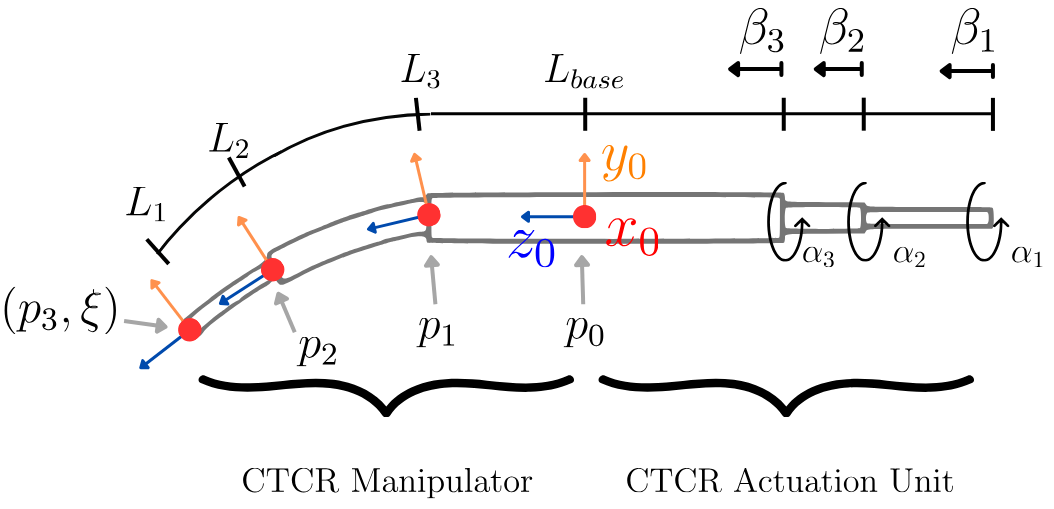
\includegraphics[width=\columnwidth]{Figures/CTCR.png}
    %}
    \caption{
    Diagram of an annotated CTCR consisting of three precurved tubes. Please note that the innermost, middle, and outermost tubes are referenced with the indices 1, 2, and 3 respectively.
    }
    \label{fig:ctcr}
\end{figure}
}

\bulletpoints{
    \item Topic Sentence: To justify the problem mentioned in the previous paragraph, this paragraph should introduce to the reader the literature on Cosserat Rod optimizations. The goal is to convince the reader that although there has been a lot of work in this area, there has been no definite, universal approach to optimize the problem.
    \item Provide a brief overview of the various efforts that have been undertaken to optimize the problem
    \item Categorize these efforts into the universal-approaches (architecture and hardware agnostic) vs system-specific approaches
    \item Discuss the level of optimization that each approach achieved and compare them.
    \item Argue that there remains a need for an optimization approach that achieves real-time control while being universal.
}

\commentblock{
Efforts to optimize the computational cost of solving the Cosserat rod model have been extensive, yet no universal approach has emerged.
While some studies offer broad, architecture-agnostic improvements, they often fall short of real-time control, achieving execution times of $40$ ms and $57$ ms respectively \cite{RuckerWebster_ICRA_2011, OrekhovSimaan_IROS_2020}.
Other optimizations achieve real-time performance but are limited by specific robot architectures \cite{TillBrysonChungOrekhovRucker_ICRA_2015} or actuation systems \cite{XuPatel_EMBC_2012}.
Despite these advancements, there remains a critical need for an optimization strategy that not only achieves real-time control but is also universally applicable, balancing generalized performance with real-time execution across various systems.
}

\bulletpoints{
    \item Topic Sentence: In this paragraph, I want to explain what our contribution to the field is. I want to discuss how we attempted to solve the problem stated above and what our final solution is. Lastly, I want to discuss our results and why they are significant (at least to me).
    \item Explain the framework/approach used to solve this problem.
    \item Discuss why the optimization strategy used ensures universality.
    \item Discuss the runtime improvement achieved and why it is significant.
    \item Discuss the potential proxy to elastic stability and why it is significant.
}

\commentblock{
This paper presents a comprehensive investigation of the numerical tools used in the computation of the static forward kinematics (FK) of CTCRs.
We introduce a variety of numerical optimization techniques that result in significant runtime reductions with no compromise in accuracy, enabling real-time performance while maintaining universal applicability across model implementations.
Additionally, we demonstrate a potential numerical proxy for assessing the robot's elastic stability which opens up new possibilities for stable path planning in CTCR systems.
}

\subsection{State of the Art}

\bulletpoints{
    \item Topic Sentence: A brief and quick introduction to the state of the art. This section should explain how the BVP is currently solved (classical RK4 with Newton-Raphson solver) and why (no need to perserve group structure, ease of use in Matlab, etc).
    \item Discuss the shooting method and why it is used to solve the BVP
    \item Briefly explain why there is no need to perserve rotation group structure.
    \item Discuss the integrator used and why it is used
    \item Discuss the solver used and why it is used
}

\commentblock{
Current state-of-the-art approaches for solving the BVP primarily use explicit Runge-Kutta methods combined with the Newton-Raphson nonlinear solver \cite{RuckerJonesWebster_TRO_2010, RuckerWebster_ICRA_2011, Gilbert_Springer_2016, Burgner-Kahrs_TRO_2015}.
This combination is favored due to its robustness and ease of use, particularly in environments like \textsc{MATLAB} \cite{RuckerJonesWebster_TRO_2010, RuckerWebster_ICRA_2011, TillBrysonChungOrekhovRucker_ICRA_2015}.
Although it was initially believed that specialized integrators were needed to preserve rotation group structure \cite{DupontLockItkowitzButler_TRO_2010}, the error from standard explicit integrators has been shown to be negligible compared to the model's inherent kinematic error \cite{Gilbert_Springer_2016, DieciRussellVanVkeck_SIAM_1994}.
The shooting method is commonly employed in this framework, effectively guiding the solution towards convergence.
}

%===============================================================================
% The Forward Kinematics
\section{THE BOUNDARY VALUE PROBLEM}

This section discusses the mathematical formulation of the BVP for CTCRs. It introduces the Cosserat rod model, examines the stiffness of the model, and reviews existing methods, setting the foundation for the computational benchmarks explored later.

\commentblock{
\begin{table}[thb!]
	\centering
	\caption*{\textsc{Nomenclature}}
	\label{tab:nomenclature}
    \resizebox{0.49\textwidth}{!}{%
        \begin{tabular}{l l}
            \hline
            \hline
            \\
    
            $\boldsymbol{a}$      & \text{Bold typeface for vectors} \\
            $A$                   & \text{Uppercase typeface for matrices} \\
            $n$                   & \text{Number of concentric, precurved tubes} \\
            $s$                   & \text{Point along the robot's arc-length} \\
            $(\cdot)^*$           & \text{Denotes that the variable is in the undeformed state} \\
            $\boldsymbol{r}_i(s)$ & \text{The position vector for tube $i$ at point $s$} \\
            $R_i(s)$              & \text{The rotation matrix for tube $i$ at point $s$} \\
            $g_i(s)$              & \text{The reference frame for tube $i$ at point $s$} \\
            $E_i$                 & \text{Young's modulus for tube $i$} \\
            $G_i$                 & \text{Shear modulus for tube $i$} \\
            $I_i$                 & \text{The second moment area for tube $i$} \\
            $J_i$                 & \text{The polar moment of inertia of the $i$th tube's cross-section} \\
            $K_i$                 & \text{Stiffness matrix for tube $i$} \\
            $(\cdot)^\vee$        & \text{Denotes the conversion from $\mathfrak{so}(3)$ or $\mathfrak{se}(3)$ to $\mathbb{R}^3$ or $\mathbb{R}^6$ respectively} \\
            $\widehat{\cdot}$     & \text{The inverse function of $(\cdot)^\vee$} \\
            $\boldsymbol{u}_i(s)$ & \text{Precurvature vector for tube $i$ at point $s$} \\
            $\theta_i$            & \text{Axial angle of the $i$th tube} \\
            $\boldsymbol{\xi}$    & \text{Rate of change of the reference frame $g$} \\
            $u_{i,z}(s)$          & \text{Torsional strains for tube $i$ at point $s$} \\ 
            $\alpha_i$            & \text{Rotational joint value corresponding to the $i$th tube} \\
            $\beta_i$             & \text{Translational joint value corresponding to the $i$th tube} \\
            $\boldsymbol{q}$      & \text{The robot's joint space vector} \\
            $L_i$                 & \text{Length of the $i$th tube} \\
            $\boldsymbol{y}$      & \text{State vector for the ODE system} \\
            $\boldsymbol{f}(s, \boldsymbol{y})$ & \text{Derivative of the state vector} \\
            $A(s)$                & \text{Jacobian matrix of the ODE system at point $s$} \\
            $\lambda_j(s)$        & \text{Eigenvalue of $A(s)$} \\
            $h$                   & \text{Integration step-size} \\
            $k$                   & \text{Non-linear solver iteration count} \\
            $n_{\boldsymbol{f}}(h)$              & \text{Denotes the number of calls to $f$ using a step-size of $h$} \\
            $e_p$                 & \text{Position error} \\
            
            \\
            \hline
            \hline
        \end{tabular}
    }
\end{table}
}

\subsection{The Cosserat Rod Model}

\bulletpoints{
    \item Topic Sentence: A brief overview of Cosserat Rod theory. This paragraph should discuss the forces it models and the simplifying assumptions made by Kirchhoff and by us in this paper.
    \item Introduce Cosserat Rod theory
    \item Cosserat Rod theory uses bend, twist, stretch, and shear to represent the 6 dof
    \item Introduce Kirchhoff assumptions
    \item Discuss our own assumptions (Constant precurvature and precurved around x-axis)
}

\commentblock{
Cosserat rod theory provides a comprehensive mathematical framework for modeling slender, one-dimensional rods by accounting for bend, twist, stretch, and shear to represent all six degrees of freedom at each cross-section \cite{RuckerJonesWebster_TRO_2010}.
In the context of CTCRs, Kirchhoff rod theory, a special case of Cosserat rod theory that assumes inextensibility and shearlessness, is used.
These assumptions are generally valid given the long, thin Nitinol tubes used in CTCRs \cite{RuckerJonesWebster_TRO_2010}.
In addition to the Kirchhoff assumptions, we will further assume that the tubes' precurvature is constant across the arc length and that the tubes are precurved solely around the x-axis as is shown in Fig.~\ref{fig:ctcr}.
}

\bulletpoints{
    \item Topic Sentence: Walk through the Cosserat Rod equations and explain how it gives rise to the ODE system.
    \item Explain how the reference frames are formed
    \item Introduce the stiffness matrix and local precurvature vector
    \item Explain how to initialize the state variables
    \item Introduce the final ODE system which forms the BVP
    \item Introduce the initial and final boundary conditions
}

\commentblock{
To model a collection of $n$ concentric, precurved tubes, we must assign homogeneous reference frames along the tubes' arc-lengths.
By convention, the $z$-axes of these frames are always tangent to the curve of the tube, resulting in the frame formulation
\begin{align*}
    g^{*}_i(s) =
    \begin{bmatrix}
		R^{*}_i(s) & \boldsymbol{r^{*}_i}(s)\\
		\boldsymbol{0}^T & 1\\
	\end{bmatrix}
    .
\end{align*}
The material properties and the tube's geometry of each cross-section can be described by the stiffness matrix $K_i$ and the local precurvature vector $\boldsymbol{u}_i(s)$ respectively:
\begin{align*}
    & K_i =
    \begin{bmatrix}
		E_iI_i & 0 & 0\\
		0 & E_iI_i & 0\\
        0 & 0 & G_iJ_i\\
	\end{bmatrix},
    & \boldsymbol{u}^{*}_i(s) =
    \begin{pmatrix}
		R^{*T}_i(s)\dot{R}^{*}_i(s)
	\end{pmatrix}^\vee &
    .
\end{align*}
Lastly, by initializing the following state variables as
\begin{align*}
    & R_{\theta_i} = \begin{bmatrix}
		\cos \theta_i & -\sin \theta_i & 0\\
		\sin \theta_i & \cos \theta_i & 0\\
        0 & 0 & 1\\
	\end{bmatrix} & K = \sum^n_{i = 1} K_i \\
    & \boldsymbol{u}_i = R^T_{\theta_i}\boldsymbol{u}_1 + \dot{\theta}_i \boldsymbol{e}_3 & \boldsymbol{\xi} = \begin{bmatrix}
		0 & 0 & 1 & \boldsymbol{u}^T_1\\
	\end{bmatrix}^T
    ,
\end{align*}
an ODE system can be constructed using the Cosserat rod equations to describe the tubes' shapes along with the elastic interactions between them:
\begin{align*}
    \dot{g} &= g\widehat{\boldsymbol{\xi}}\\
    \dot{\theta}_i &= u_{i, z} - u_{1, z}\\
    \begin{bmatrix}
		\dot{u}_{1, x}\\
		\dot{u}_{1, y}\\
	\end{bmatrix} &= -K^{-1}(\sum^{n}_{i=1} R_{\theta_i}(K_i (\dot{\theta}_i \frac{dR^T_{\theta_i}}{d\theta_i}\boldsymbol{u}_1) \\
    & + \widehat{\boldsymbol{u}}_i K_i (\boldsymbol{u}_i - \boldsymbol{u}^{*}_i)) + \widehat{e}_3 R^T_1 \boldsymbol{w}_f)|_{x, y}\\
    \dot{u}_{i, z} &= \frac{E_iI_i}{G_iJ_i}(u_{i, x}u^{*}_{i, y} - u_{i, y}u^{*}_{i, x})
    .
\end{align*}
With constant tube precurvature and zero z-axis curvature, the final boundary condition simplifies to zero torsional strains $u_{i, z}$ at each tube's end.
The initial boundary condition at $s = 0$ relates to the robot's joint space and is defined as:
\begin{align*}
    & \boldsymbol{r}(0) = \begin{bmatrix}
		0 & 0 & 0\\
	\end{bmatrix}^T & \theta_1 = \alpha_1 - \beta_1 u_{1, z} \\
 & \theta_i = (\alpha_i - \beta_i u_{i, z}) - \theta_1, \quad i \geq 2
 .
\end{align*}
}

\subsection{Stiffness Analysis of the BVP}

\bulletpoints{
    \item Topic Sentence: Define the ODE system and the jacobian matrix $A(s)$. Briefly explain BVP stiffness.
    \item Define $A(s)$ using $f(s, y)$ and using the state variables
    \item Introduce the BVP criterion for stiffness
    \item Compare BVP stiffness to IVP stiffness and explain the effect of boundary conditions on solution divergence.
    \item Establish the need to determine an upper bound for the eigenvalues.
}

\commentblock{
\begin{figure*}[t!]
    \normalsize

    \begin{align*}
        A(s) = \begin{bmatrix}
                0 & \cdots & 0 & 0 & 0 & -1 & 1 & \cdots & 0\\
                \vdots & \ddots & \vdots & \vdots & \vdots & \vdots & \vdots & \ddots & \vdots\\
                0 & \cdots & 0 & 0 & 0 & -1 & 0 & \cdots & 1\\
                \frac{\partial f_n}{\partial y_1} & \cdots & \frac{\partial f_n}{\partial y_{n-1}} & \frac{\partial f_n}{\partial y_n} & \frac{\partial f_n}{\partial y_{n+1}} & \frac{\partial f_n}{\partial y_{n+2}} & \frac{\partial f_n}{\partial y_{n+3}} & \cdots & \frac{\partial f_n}{\partial y_{2n+1}} \\
                \frac{\partial f_{n+1}}{\partial y_1} & \cdots & \frac{\partial f_{n+1}}{\partial y_{n-1}} & \frac{\partial f_{n+1}}{\partial y_n} & \frac{\partial f_{n+1}}{\partial y_{n+1}} & \frac{\partial f_{n+1}}{\partial y_{n+2}} & \frac{\partial f_{n+1}}{\partial y_{n+3}} & \cdots & \frac{\partial f_{n+1}}{\partial y_{2n+1}} \\
                0 & \cdots & 0 & \frac{\partial f_{n+2}}{\partial y_n} & \frac{\partial f_{n+2}}{\partial y_{n + 1}} & 0 & 0 & \cdots & 0 \\
                \frac{\partial f_{n+3}}{\partial y_1} & \cdots & 0 & \frac{\partial f_{n+3}}{\partial y_n} & \frac{\partial f_{n+3}}{\partial y_{n + 1}} & 0 & 0 & \cdots & 0 \\
                \vdots & \ddots & \vdots & \vdots & \vdots & \vdots & \vdots & \ddots & \vdots\\
                0 & \cdots & \frac{\partial f_{2n+1}}{\partial y_{n-1}} & \frac{\partial f_{2n+1}}{\partial y_n} & \frac{\partial f_{2n+1}}{\partial y_{n + 1}} & 0 & 0 & \cdots & 0 \\
        \end{bmatrix}
    \end{align*}

    \caption*{The analytical Jacobian of the non-linear ODE presented in Eq.~\ref{eq:ode_system}.}
    \label{eq:analytical_Jacobian}
\end{figure*}

The stiffness of an ODE system indicates its conditioning.
Stiff ODEs require the use of implicit integrators and/or minuscule step sizes to prevent divergence, while non-stiff ODEs allow the use of explicit integrators with moderate step sizes \cite{AscherPetzold_SIAM_1998, Heath_SIAM_2018}.
Consider the BVP described by the following non-linear ODE system
\begin{align}
    \label{eq:ode_derivative}
    \dot{\boldsymbol{y}} = \boldsymbol{f}(s, \boldsymbol{y}), \quad 0 \leq s \leq b\\
    A(s) = \frac{\partial \boldsymbol{f}}{\partial \boldsymbol{y}}(s, \boldsymbol{y})
    \label{eq:ode_system}
    ,
\end{align}
where $A(s) \in \mathbb{R}^{m \times m}$.
A BVP is considered stiff if and only if
\begin{align*}
    b|\Re(\lambda_j(s))| \gg 1, \quad 1 \leq j \leq m
    ,
\end{align*}
\cite{AscherPetzold_SIAM_1998}.
Unlike IVPs, BVP stiffness depends on boundary conditions, allowing it to tolerate error accumulation from positive eigenvalues if the integration interval near the final boundary $b$ is small enough \cite{AscherPetzold_SIAM_1998}.
}

\bulletpoints{
    \item Topic Sentence: Lay down the foundations for the statistically derived upper-bound.
    \item Define the state vector for the ODE system
    \item Finding an analytical upper bound is tough, that is why we sampled 20 million configurations.
    \item The The configurations were sampled uniformly and the maximum over the interval was calculated
}

\commentblock{
Following \cite{RuckerWebster_ICRA_2011}, we define our state $\boldsymbol{y}$ as
\begin{align}
    \boldsymbol{y} &= [\theta_2, \cdots, \theta_n, u_{1, x}, u_{1, y}, u_{1, z}, u_{2, z}, \cdots, u_{n, z}]^T\\
	&= [y_1, \cdots, y_{n - 1}, y_n, y_{n + 1}, y_{n + 2}, y_{n + 3}, \cdots, y_{2n + 1}]^T
    \label{eq:state_variables}
\end{align}
where the first $n - 1$ elements determine the position and orientation at $s$, and the remaining elements describe tube bending and torsion \cite{RuckerJonesWebster_TRO_2010}.
Deriving an analytical upper bound for the eigenvalues of $A(s)$ is challenging due to the non-linear relationships between the state variables.
Instead, we employed a statistical approach, sampling $20,000,000$ configurations uniformly and calculating the maximum $max(|\Re(\lambda_j(s))|)$ across the integration interval. 
}

\bulletpoints{
    \item Topic Sentence: Discuss the upper-bound used and how it satisfies the criterion.
    \item The upper bound used is 20 because it is really improbably that the eigenvalues will be higher.
    \item Using 20 as the upper bound and b = 0.21, the criterion is satisfied.
    \item Yeah, this might seem sketchy but it is safe to assume it's not
}

\commentblock{
\begin{figure}
    %\fbox{
    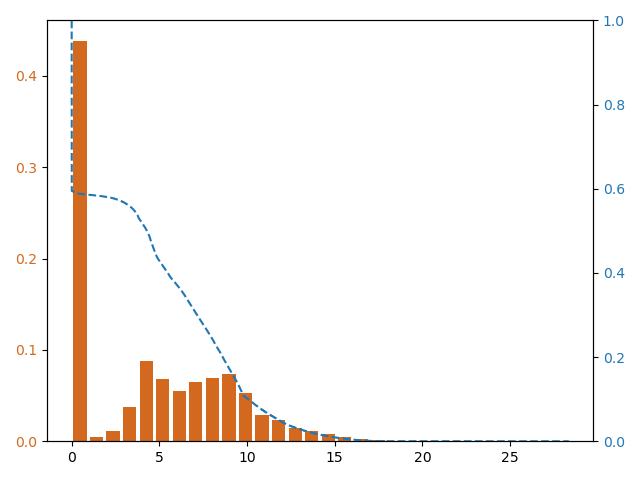
\includegraphics[width=\columnwidth]{Figures/max eigen_histogram.png}
    %}
    \caption{
    Histogram of the sampled $max(|\Re(\lambda_j(s))|)$. The orange bars represent the density while the blue line represents the empirical complementary cumulative distribution function (CCDF). A total of $20,000,000$ configurations were sampled.
    }
    \label{fig:eigen_distribution}
\end{figure}

We use $20$ as the upper bound for the system's eigenvalues since $|\Re(\lambda_j(s))| > 20$ has only a $0.001\%$ probability of occurrence, as can be seen in Fig. ~\ref{fig:eigen_distribution}.
With a maximum CTCR arc length of 210 mm, we assume
\begin{align*}
    0 \leq |\Re(\lambda_j(s))| \leq 20\\
    0 \leq b|\Re(\lambda_j(s))| \leq 4.2
\end{align*}
where $b=0.21$, indicating that the BVP is non-stiff.
While the aforementioned, approximated eigenvalue upper-bound is specific to the CTCR parameters used, the widespread success of using the shooting method with the explicit classical Runge-Kutta integrators \cite{Burgner-Kahrs_TRO_2015} suggests that the BVP is generally non-stiff.
}

%===============================================================================
% Methods
\section{METHODS}

In this section, we explore the numerical methods applied to optimize the static FK of CTCRs. The focus is on numerical integration techniques, orientation representations, and solver strategies, all aimed at improving computational efficiency.

\subsection{Numerical Integration}

\bulletpoints{
    \item Topic Sentence: Compare and contrast RK integrators with AB integrators. Briefly explain the theory behind both to show why AB is more efficient.
    \item Explain how RK integrators work
    \item Discuss RK computational cost
    \item Explain how AB integrators work
    \item Discuss AB computational cost
    \item Discuss the stability region of AB methods and how extrapolation affects it
}

\commentblock{
An $\stage$-stage Runge-Kutta (RK) method uses an interpolating polynomial of degree $\stage$
\begin{align*}
	\boldsymbol{Y}_i &= \boldsymbol{y}_{n-1} + h \sum_{j=1}^{i} a_{ij} \boldsymbol{f}(s_{n-1} + c_j h, \boldsymbol{Y}_j )\\
	\boldsymbol{y}_n &= \boldsymbol{y}_{n-1} + h \sum_{i=1}^{\stage} b_i \boldsymbol{f}(s_{n-1} + c_i h, \boldsymbol{Y}_i)
\end{align*}
requiring $\stage$ function evaluations per step \cite{AscherPetzold_SIAM_1998}.
In contrast Adams-Bashforth (AB) integrators extrapolate the solution using previous integration steps, requiring only one new function evaluation per step resulting in a comparable performance to Forward Euler (FE) \cite{AscherPetzold_SIAM_1998}.
Nonetheless, the stability region decreases with higher-degree extrapolation, limiting AB methods to problems with low stiffness \cite{AscherPetzold_SIAM_1998, Heath_SIAM_2018}.
The extrapolating polynomial for an $\stage$-stage AB method is constructed as follows
\begin{align*}
    \boldsymbol{y}_n = \boldsymbol{y}_{n - 1} + h \sum^{\stage}_{j = 1} \gamma_j \boldsymbol{f}(s_{n - j}, \boldsymbol{y}_{n - j})
    ,
\end{align*}
where $\gamma_j$ is the coefficient at each interpolating point.

\begin{table}[thb!]
	\centering
	\caption{Coefficients of AB methods up to order 5 \cite{AscherPetzold_SIAM_1998}.}
	\label{tab:adams_bashforth}
    \begin{tabular}{c || c | ccccc}
    $\stage$         & $j \rightarrow$  & $1$    & $2$     & $3$    & $4$     & $5$  \\
    \hline
    $1$         & $\gamma_j$       & $1$ \\
    $2$         & $2\gamma_j$      & $3$    & $-1$ \\
    $3$         & $12\gamma_j$     & $23$   & $-16$   & $5$ \\
    $4$         & $24\gamma_j$     & $55$   & $-59$   & $37$   & $-9$\\
    $5$         & $720\gamma_j$    & $1901$ & $-2774$ & $2616$ & $-1274$ & $251$\\
    \end{tabular}
\end{table}
}

\subsection{Integrating Orientation}

\bulletpoints{
    \item Topic Sentence: Introduce quaternions. Explain that it was initially though to degrade $SO(3)$ structure.
    \item Define quaternions
    \item Explain that quaternions provide a minimal rotation description, making it computationally efficient.
    \item Quaternions were though to degrade $SO(3)$ during integration and unit-length was enforced which negates the computational benefits.
    \item With the quaternion derivative equation, standard integrators can be used along with the derivative equation without degrading $SO(3)$ structure
}

\commentblock{
A quaternion is a hyper-complex number represented as
\begin{align*}
    \boldsymbol{\eta} = a + b\boldsymbol{i} + c\boldsymbol{j} + d\boldsymbol{k},\\
    \boldsymbol{i}^2 = \boldsymbol{j}^2 = \boldsymbol{k}^2 = \boldsymbol{ijk} = -1,
\end{align*}
with real coefficients $a, b, c, d$ for the basis vectors $\boldsymbol{1}, \boldsymbol{i}, \boldsymbol{j}, \boldsymbol{k}$ \cite{Stuelpnagel_SIAM_1964}.
Quaternions offer a minimal yet complete 3D rotation description, making them a computationally efficient representation of $SO(3)$ \cite{Stuelpnagel_SIAM_1964}.
Initially, it was believed that integrating non-unit quaternions would degrade the $SO(3)$ structure, requiring the enforcement of unit length as an additional algebraic constraint, which was computationally intensive \cite{Rucker_RAL_2018}.
However, \cite{Rucker_RAL_2018} showed that non-unit quaternions can be integrated without constraints using the conventional quaternion derivative equation
\begin{align*}
    & \boldsymbol{\dot{\eta}} = \frac{1}{2} W^T \boldsymbol{\omega}, & W = \begin{bmatrix}
		-b &  a &  d & c \\
		-c & -d &  a & b \\
        -d &  c & -b & a \\
	\end{bmatrix} &
\end{align*}
where $\omega \in \mathbb{R}^3$ is the body-frame's angular velocity vector, significantly improving accuracy over to Euler angles and rotation matrices \cite{Rucker_RAL_2018, GrassmanBurgner-Kahrs_RSS_2019}.
}

\subsection{Non-Linear Solvers}

\bulletpoints{
    \item Topic Sentence: Introduce the Newton Raphson algorithm and compare finite differences to secant
    \item Define and explain how Newton Raphson works
    \item Newton method achieves quadratic convergence but convergence is not guaranteed
    \item Finite differences needs $m + 1$ function evaluations along with $\mathcal{O}(m^3)$ arithmetic operations to get the inverse.
}

\commentblock{
Let $\boldsymbol{z}: \mathbb{R}^m \rightarrow \mathbb{R}^m$ be a differentiable function with $D(\boldsymbol{x})$ as its Jacobian matrix.
Iteratively solving $D(\boldsymbol{x})\boldsymbol{d} = -\boldsymbol{z}(\boldsymbol{x})$ using the Newton-Raphson method converges towards a local minimum, corresponding to a root of $\boldsymbol{z}$ \cite{Heath_SIAM_2018}.
Newton-Raphson achieves quadratic convergence, doubling the number of correct digits with each iteration \cite{Heath_SIAM_2018}.
However, convergence is not guaranteed if $D$ is singular, $\boldsymbol{z}$ is poorly conditioned, or no root exists.
Without a closed-form expression, computing $D$ can be costly since approximating $D$ via finite differences requires at least $m + 1$ evaluations of $\boldsymbol{z}$ per iteration, and solving the linear system involves $\mathcal{O}(m^3)$ arithmetic operations, adding significant computational overhead \cite{Heath_SIAM_2018}.

\begin{algorithm}
    \begin{algorithmic}[1]
        \State $\boldsymbol{x_0} \gets$ initial guess
        \For{$k = 1,2,3,\dots$}
            \State Solve $D(\boldsymbol{x}_{k - 1})\boldsymbol{d} = -\boldsymbol{z}(\boldsymbol{x}_{k - 1})$ for $\boldsymbol{d}$
            \State $\boldsymbol{x}_k \gets \boldsymbol{x}_{k - 1} + \boldsymbol{d}$
        \EndFor
    \end{algorithmic}
    \caption{Newton-Raphson's Method}
    \label{alg:newton}
\end{algorithm}
}

\bulletpoints{
    \item Topic Sentence: Introduce and explain Broyden's multi-dimensional secant update.
    \item Secant update is computationally inexpensive and is a good enough approximation for well-conditioned problems.
    \item Although secant update achieves super-linear convergence, it can still achieve a better runtime if finite differences are really expensive
    \item Broyden extended the secant update to multiple dimensions
    \item Broyden used the Sherman-Morrison formula to update the inverse jacobian directly
}

\commentblock{
In one-dimensional problems, the secant update offers a computationally inexpensive alternative to finite-differences for derivative approximations, especially when $\boldsymbol{z}(x)$ is well-conditioned but costly to compute.
Despite the secant method's super-linear convergence rate of $(1 + \sqrt{5})/2 \approx 1.618$, its lower cost per iteration often outweighs the slightly higher number of iterations needed \cite{Heath_SIAM_2018}.
In \cite{Broyden_AMS_1965}, Broyden extended the secant method to multiple dimensions by directly updating the Jacobian matrix using rank-one updates
\begin{align}
    D_k = D_{k - 1} + \frac{\Delta \boldsymbol{z}_k - D_{k - 1} \Delta \boldsymbol{x}_k}{\|\Delta \boldsymbol{x}_k\|^2} \Delta \boldsymbol{x}^T_k
    .
    \label{eq:secant_update_broyden}
\end{align}
He also noted that the Sherman–Morrison formula (Eq.~\ref{eq:sherman-morrison}) can be used to directly update the inverse Jacobian matrix $D^{-1}$
\begin{align}
    (U + \boldsymbol{u}\boldsymbol{v}^T)^{-1} = U^{-1} - \frac{U^{-1} \boldsymbol{u}\boldsymbol{v}^T U^{-1}}{\boldsymbol{1} + \boldsymbol{v}^T U^{-1}\boldsymbol{u}}
    \label{eq:sherman-morrison}
\end{align}
where, for some vectors $\boldsymbol{u}, \boldsymbol{v} \in \mathbb{R}^m$, $\boldsymbol{u}\boldsymbol{v}^T$ is the outer product \cite{Broyden_AMS_1965}.
Applying the Sherman-Morrison formula to Broyden's multi-dimensional secant update (Eq.~\ref{eq:secant_update_broyden}) results in
\begin{align}
    D^{-1}_k = D^{-1}_{k - 1} - \frac{\boldsymbol{d}_k \left(-\boldsymbol{d}^T_{k - 1} D^{-1}_{k-1} \right)^T}{-\boldsymbol{d}_{k - 1}^T (\boldsymbol{d}_k - \boldsymbol{d}_{k - 1})}
    \label{eq:inverse_Jacobian_update}
\end{align}
where $\boldsymbol{d}_k = D^{-1}_{k - 1} \boldsymbol{z}_k$ is the gradient at iteration $k$ \cite{Misha_Lecture}.
Please note that the fraction notation implies element-wise or Hadamard division \cite{Broyden_AMS_1965}.
}

\bulletpoints{
    \item Topic Sentence: Explain the computational complexity of the Broyden update
    \item Allows for direct gradient calculation, each update requires only $\mathcal{O}(m^2)$ operations per iteration
    \item Only needs a single function call per iteration to calculate $D^{-1}$.
}

\commentblock{
The availability of the inverse Jacobian allows for direct gradient calculation, with each secant update requiring only $\mathcal{O}(m^2)$ operations per iteration \cite{Heath_SIAM_2018}.
Moreover, employing the secant update method reduces the number of function calls to $\boldsymbol{z}$ from $m + 1$ calls to a single function call per iteration, significantly lowering the computational cost to a level comparable to having a closed-form of $D^{-1}$.
}

\subsection{Inverse Jacobian Initialization}

\bulletpoints{
    \item Topic Sentence: When initializing the inverse jacobian, an approximation can be used to lower the computational cost.
    \item Explain how different levels of approximations work (the two extremes: identity matrix or finite differences).
    \item We can use a larger step-size when initializing the jacobian
    \item The optimal initial step size can be obtained by applying a minimization function.
}

\commentblock{
Multi-dimensional secant updates typically begin by initializing $D^{-1}$, often via finite-differences, which can be costly if the iteration count is low.
Alternatively, using the identity matrix for $D^{-1}$ might work for well-conditioned problems but may require a higher iteration count to correct the poor initial estimate \cite{Heath_SIAM_2018}.
In this context, varying the initial step size $h_{\text{initial}}$ used in the Jacobian construction can provide control over the approximation level present, with larger $h_{\text{initial}}$ resulting in rougher estimates.
To minimize total function calls while solving the BVP, the optimal $h_{\text{initial}}$ can be determined using
\begin{align}
    h_{\text{optimal}} = \underset{h_\text{initial}}{\operatorname{argmin}} \left( n_{\boldsymbol{f}}(h) + n_{\boldsymbol{f}, D}(h_{\text{initial}}) \right)
    \label{eq:minimization_criterion}
\end{align}
where $n_{\boldsymbol{f}, D}(h_{\text{initial}})$ is the number of function calls used to approximate $D^{-1}$.
}

%===============================================================================
% Evaluation
\section{EVALUATION}

This section evaluates the performance and accuracy of the CTCR model. It presents the calibration of the CTCR model, followed by a discussion of the sampling method used and the specifics of the model's implementation.

\subsection{Model Implementation}

\bulletpoints{
    \item Topic Sentence: Discuss the programming specifics with respect to the model implementation
    \item Implemented using C++ with g++ compiler.
    \item Compiler flags were -O3 and -march=native
    \item Float64 was used over double datatype and the chrono library was used for measuring runtime.
    \item Describe the specs of the system used
}

\commentblock{
The Cosserat rod static model, outlined in \cite{RuckerJonesWebster_TRO_2010}, was implemented in \textsc{C++} and compiled with the g++ compiler.
The \texttt{-O3} compiler flag was used for the maximum \textsc{IEEE} compliant runtime speed optimization and the \texttt{-march=native} flag was used to optimize for the specific processor architecture available.
The \texttt{\_Float64} data type was preferred over \texttt{double} for enhanced floating-point processing.
Time measurements for solving the forward kinematics were made using \textsc{C++}'s \texttt{chrono} library, which offers nanosecond precision.
Computations were performed on a 64-bit \textsc{Linux} system with a Ryzen-5 3500-U \SI{2.1}{GHz} 4-core, 8-thread processor.
}

\bulletpoints{
    \item Topic Sentence: Discuss the methods specifics with respect to the model implementation
    \item Step-size was 1mm for all integrators. Zero initial forces was the default guess for all solvers.
    \item Ralston's coefficients were used for RK integrators.
    \item Ground truth values were obtained using a step size of 10 micrometers, Newton solver, RK4, and rotation matrices
    \item Broyden update and AB2 were used for parameter calibration and eigenvalue data
}

\commentblock{
A constant step-size of \SI{1}{mm} is used in all integrators with zero initial forces as the default guess for all solvers.
The Ralston's coefficients for RK integrators were used since they provide the lowest possible truncation error \cite{Ralston_AMS_1962}. 
Ground-truth values were calculated using the Newton-Raphson non-linear solver and the fourth-order RK integrator with a \SI{10}{\mu m} step size, using rotation matrices for orientation.
For eigenvalue data collection (Fig.~\ref{fig:eigen_distribution}) and parameter calibration (Fig.~\ref{fig:pos_err_distribution}), the model used Broyden's update method with the second-order AB integrator.
}

\bulletpoints{
    \item Topic Sentence: Discuss the sampling method used
    \item Each model combo was evaluated on 1 million random samples.
    \item Introduce and explain Reinhard's sampling method.
}

\commentblock{
Each model type, defined by a unique combination of numerical methods, was evaluated on $1,000,000$ random samples, with the averaged results shown in Table~\ref{tab:results}.
To disentangle the $\beta_i$ values and provide a truly uniform sampling of the workspace, the transformation matrix
\begin{align*}
	M_{\mathcal{B}}
	=
	\begin{bmatrix}
		- L_1	&	        0   &	        0\\
		- L_1	&	L_1 - L_2   &	        0\\
		- L_1	&	L_1 - L_2   &	L_2 - L_3\\
	\end{bmatrix}    
\end{align*}
can be used, providing an efficient and bias-free sampling technique \cite{GrassmannSenykBurgner-Kahrs_ICRA_2024}:
\begin{align*}
    \begin{bmatrix}
        \beta_1\\
        \beta_2\\
        \beta_3\\
	\end{bmatrix} = \frac{1}{2} \begin{bmatrix} M_{\mathcal{B}} & M_{\mathcal{B}} \cdot \boldsymbol{1}_{3 \times 1} \\ \end{bmatrix}
    \begin{bmatrix}
        \mathcal{U}[-1;1] \\
		\mathcal{U}[-1;1] \\
		\mathcal{U}[-1;1] \\
        1
	\end{bmatrix}.
\end{align*}
}

\subsection{Model Calibration}

\bulletpoints{
    \item Topic Sentence: Introduce the dataset used for calibration and discuss its specifics
    \item The CTCR model used the same parameters as the robot from the dataset
    \item Describe how the configurations were collected and the size of the dataset
    \item The least squares problem was run on 10k data points
    \item Explain how the least squares problem was set up
}

\commentblock{
\begin{figure}[t!]
    \centering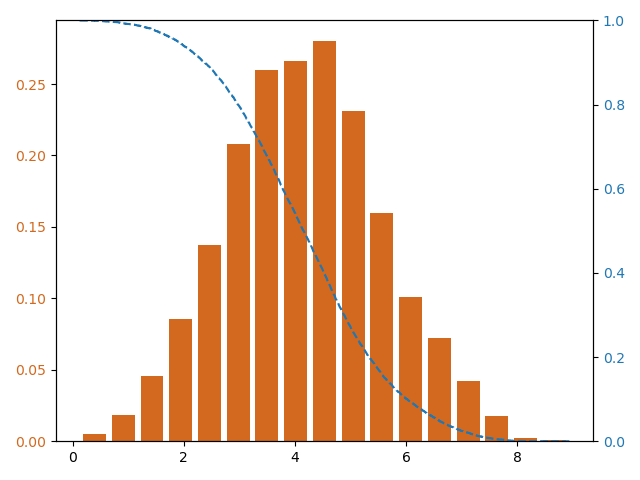
\includegraphics[width=\columnwidth]{Figures/dataset_histogram.png}
	\caption{
        Histogram of the tip errors $e_p(L_3)$ after calibration. Orange bars indicate the density while the blue line represents the empirical CCDF. Calibration on $10,000$ random data points resulted in a mean of $4.172 \pm 1.394$ \si{mm} and a median of $4.155$ \si{mm}.
    }
    \label{fig:pos_err_distribution}
\end{figure}

To evaluate the model's performance and ensure correctness, the CTCR model used for data collection was based on the robot parameters used by Grassmann et al. \cite{GrassmanChenLiangBurgner-Kahrs_IROS_2022}.
The authors used an \textsc{Aurora} v2 electromagnetic tracking system to collect a dataset of $100,000$ robot configurations, including position vectors and quaternions for the distal ends, $L_\text{base}$, $L_3$, $L_2$, and $L_1$ in the tracking system's reference frame.
The dataset is available under an open license.
The robot's parameters (Table ~\ref{tab:robot_parameters}) were calibrated by solving a non-linear least squares problem using $10,000$ randomly selected data points.
An offset vector $\boldsymbol{\delta_p}$ was applied to the distal end positions to reduce sensor placement uncertainty, and these adjusted positions were then transformed to the robot's base frame.
The optimization function was specified as
\begin{align*}
    & \boldsymbol{P} = \begin{bmatrix}
        \boldsymbol{\delta}_{p, L_\text{base}}^T & \boldsymbol{\delta}_{p, L_3}^T & \boldsymbol{\delta}_{p, L_2}^T & \boldsymbol{\delta}_{p, L_1}^T
    \end{bmatrix}^T \\
    & \boldsymbol{P}_{\text{optimal}} = \underset{\boldsymbol{P}}{\operatorname{argmin}} \left( e_{p}(L_1) + e_{p}(L_2) + e_{p}(L_3) \right)
\end{align*}
where $e_p = \|\boldsymbol{r}_{\text{model}}(s) - \boldsymbol{r}_{\text{data}}(s) \|_2$.
Calibration was performed using the Trust Region Reflective (TRF) algorithm via \textsc{Scipy}'s \texttt{optimize.least\_squares} function.

\begin{table}[thb!]
	%\vspace*{-4mm}
	\centering
	\caption{Tube Parameters of the CTCR from \cite{GrassmanChenLiangBurgner-Kahrs_IROS_2022}.}
	\label{tab:robot_parameters}
	\begin{tabular}{@{} lll r r r @{}}
		\toprule
		\multicolumn{3}{c}{Parameter}
		& \multicolumn{3}{c}{Tubes$^1$}\\
		\cmidrule(r){1-3}
		\cmidrule(l){4-6}
		\multicolumn{1}{c}{Term}
		& \multicolumn{1}{c}{Symbol}
		& \multicolumn{1}{c}{Unit}
		& \multicolumn{1}{c}{inner}
		& \multicolumn{1}{c}{middle}
		& \multicolumn{1}{c}{outer}\\
		\cmidrule(r){1-1}
		\cmidrule(lr){2-2}
		\cmidrule(lr){3-3}
		\cmidrule(lr){4-4}
		\cmidrule(lr){5-5}
		\cmidrule(l){6-6}
	    Length, overall		    & $L$				& \si{mm} 		& \num{210} 	&    \num{165} 	&     \num{110} 	\\
	    Length, straight	    & $L_\mathrm{s}$	& \si{mm} 		& \num{41} 	&    \num{100} 	&     \num{100} 		\\
	    Curvature$^2$ 			& $\kappa_x$		& \si{m}$^{-1}$ 	& \num{28} 	&    \num{12.4} &     \num{4.37}	\\
	    Diameter, outer$^2$		& $d_\text{outer}$	& \si{mm} 		& \num{0.5} 	&    \num{0.9} 	&     \num{1.5}		\\
	    Diameter, inner$^2$		& $d_\text{inner}$	& \si{mm} 		& \num{0.4} 	&    \num{0.7} 	&     \num{1.2}		\\
	    Young's Modulus		    & $E$				& \si{GPa} 		& \num{50} 		&    \num{50} 	&     \num{50} 		\\
	    Poisson's ratio		    & $\nu$				& \num{1} 		& \num{0,3} 	&    \num{0,3} 	&     \num{0,3}		\\
		\bottomrule
	\end{tabular}
	\hspace*{5mm}
	\begin{enumerate}
		\item[$^1$]\hspace{-2.5mm} The inner, middle, and outer tubes are referenced to 1, 2, and 3, respectively.
		\item[$^2$]\hspace{-2.5mm} The tube diameters and curvature are taken from the manufacturer's data sheet.
	\end{enumerate}
\end{table}
}


\bulletpoints{
    \item Topic Sentence: Discuss the results of the calibration and how it compares to the literature
    \item What is the average position error?
    \item Is the data obtained consistent with the literature?
    \item How can these results be improved?
}

\commentblock{

The average tip position error was $4.172$ \si{mm} which is $1.99\%$ of the total arc length.
Approximately $92.7\%$ of the tip errors were below $6.3$ \si{mm}, or $3\%$ of the total arc length, which is consistent with the literature \cite{Burgner-Kahrs_TRO_2015, Gilbert_Springer_2016}.
Further fine-tuning of the position error can be achieved by calibrating the stiffness matrix values, as discussed in \cite{RuckerJonesWebster_TRO_2010}.

\begin{table}[H]
	\centering
	\caption{Values of Calibrated Parameters}
	\label{tab:lst_sqrs}
	\begin{tabular}{l r r r}
		\toprule
		\multicolumn{1}{c}{Tube End}
		& \multicolumn{1}{c}{$\delta x$ in \si{mm}}
		& \multicolumn{1}{c}{$\delta y$ in \si{mm}}
		& \multicolumn{1}{c}{$\delta z$ in \si{mm}} \\
		\cmidrule(r){1-1}
		\cmidrule(lr){2-2}
		\cmidrule(lr){3-3}
		\cmidrule(lr){4-4}
	    $L_\text{base}$ & \num{2.179} & \num{11.264} & \num{1.006} \\
	    $L_3$ & \num{1.844} & \num{-0.184} & \num{0.504} \\
	    $L_2$ & \num{-0.523} & \num{-4.690} & \num{-1.321} \\
	    $L_1$ & \num{-3.501} & \num{-6.389} & \num{-0.177} \\
		\bottomrule
	\end{tabular}
\end{table}

\begin{table*}
	\centering
	\caption{Average Performance of Different Numerical Models}
	\label{tab:results}
	\begin{tabular}{r rrrr rrrr rrrr}
		\toprule
		& \multicolumn{4}{c}{Newton -- Rotation Matrix}
		& \multicolumn{4}{c}{Broyden -- Rotation Matrix}
        & \multicolumn{4}{c}{Broyden -- Quaternion}\\
		\cmidrule(lr){2-5}
		\cmidrule(lr){6-9}
		\cmidrule(l){10-13}
		\multicolumn{1}{c}{\hfill  Integrator}
		& \multicolumn{1}{c}{$e_p$ in \si{mm}}
		& \multicolumn{1}{c}{$n_{\boldsymbol{f}}$}
		& \multicolumn{1}{c}{$k$}
		& \multicolumn{1}{c}{$t$ in $\mu$\si{s}}
		& \multicolumn{1}{c}{$e_p$ in \si{mm}}
		& \multicolumn{1}{c}{$n_{\boldsymbol{f}}$}
		& \multicolumn{1}{c}{$k$}
		& \multicolumn{1}{c}{$t$ in $\mu$\si{s}}
		& \multicolumn{1}{c}{$e_p$ in \si{mm}}
		& \multicolumn{1}{c}{$n_{\boldsymbol{f}}$}
		& \multicolumn{1}{c}{$k$}
		& \multicolumn{1}{c}{$t$ in \si{\mu s}}\\
		\cmidrule(r){1-1}
		\cmidrule(lr){2-2}
		\cmidrule(lr){3-3}
		\cmidrule(lr){4-4}
		\cmidrule(lr){5-5}
		\cmidrule(lr){6-6}
		\cmidrule(lr){7-7}
		\cmidrule(lr){8-8}
		\cmidrule(lr){9-9}
		\cmidrule(lr){10-10}
		\cmidrule(lr){11-11}
		\cmidrule(lr){12-12}
		\cmidrule(l){13-13}
    FE              & $2.302$ & $1790$ & $4.36$ & $\mathbf{305}$ 
                    & $2.302$ & $963$  & $\mathbf{5.12}$ & $\mathbf{164}$
                    & $2.229$ & $\mathbf{963}$  & $5.13$ & $\mathbf{155}$ \\
    AB 2	        & $2.041$ & $\mathbf{1787}$ & $\mathbf{4.35}$ & $327$  
                    & $2.039$ & $\mathbf{962}$  & $\mathbf{5.12}$ & $184$ 
                    & $2.037$ & $\mathbf{963}$  & $5.13$ & $172$ \\
    AB 3      	    & $2.034$ & $1788$ & $\mathbf{4.35}$ & $348$ 
                    & $2.034$ & $963$  & $5.13$ & $191$ 
                    & $2.028$ & $\mathbf{963}$  & $5.13$ & $182$ \\
    AB 4        	& $2.035$ & $1790$ & $4.36$ & $374$ 
                    & $2.035$ & $963$  & $\mathbf{5.12}$ & $204$ 
                    & $2.029$ & $\mathbf{963}$  & $5.13$ & $200$ \\
    AB 5        	& $2.035$ & $1789$ & $\mathbf{4.35}$ & $405$ 
                    & $2.035$ & $964$  & $5.13$ & $217$ 
                    & $2.028$ & $\mathbf{963}$  & $5.13$ & $212$ \\
    RK 2        	& $2.027$ & $3575$ & $\mathbf{4.35}$ & $537$ 
                    & $2.027$ & $1924$ & $5.13$ & $292$ 
                    & $\mathbf{2.025}$ & $1925$ & $\mathbf{5.12}$ & $288$ \\
    RK 3        	& $2.025$ & $5366$ & $4.36$ & $785$ 
                    & $\mathbf{2.025}$ & $2889$ & $5.13$ & $426$ 
                    & $\mathbf{2.025}$ & $2887$ & $5.13$ & $413$ \\
    RK 4        	& $\mathbf{2.024}$ & $7151$ & $\mathbf{4.35}$ & $1032$ 
                    & $\mathbf{2.025}$ & $3851$ & $5.13$ & $558$ 
                    & $\mathbf{2.025}$ & $3847$ & $\mathbf{5.12}$ & $541$ \\

		\bottomrule
	\end{tabular}
	%https://tex.stackexchange.com/questions/112343/beautiful-table-samples
\end{table*}
}

\subsection{Computational Benchmark}

\bulletpoints{
    \item Topic Sentence: The benchmark used to evaluate the level of optimization is the number of function calls and runtime. This is because this combination captures minute improvements and is easier to work with.
    \item Function calls will be the benchmark along with runtime
    \item The other methods of assessing computational complexity are flawed due to their failure of capturing intricate interactions (e.g. quaternion constant runtime improvement).
    \item Butter up the reader and tell him that we are using a practical metric.
}

\commentblock{
In this paper, the primary benchmark for measuring computational complexity will be a combination of the number of function calls to $\boldsymbol{f}(s, \boldsymbol{y})$ and computational runtime.
While other methods, such as asymptotic complexity analysis and runtime measurements alone, have their merits, they often fall short in capturing the intricate interactions involved in optimization, such as constant runtime improvements due to quaternion representation.
By focusing on function call count and runtime, we provide a more accurate and accessible metric that directly reflects the optimization level achieved.
}

\subsection{Results}

\bulletpoints{
    \item Topic Sentence: Compare and contrast the performance of the different solvers.
    \item 99.8\% of all sample configurations converged successfully. The position error between Newton and Broyden was non-existent
    \item The broyden update reduced the number of function calls by 54\%
    \item The difference in accuracy between RK and AB methods is 16 micrometers, making it negligible for practical purposes.
    \item Using quaternion rotations lowered the error slightly and lowered runtime by 5\%
}

\commentblock{
Across all model types, the iteration count remained relatively low with $99.8\%$ of all sampled configurations converging successfully.
The position error was virtually identical between Newton and Broyden non-linear solvers; nonetheless, the Broyden update method reduced function calls by about $54\%$.
Although using RK integrators resulted in a slightly more accurate solution when compared to AB methods, the difference in the position error was \SI{16}{\mu m} on average making it negligible for practical purposes.
With a $5\%$ reduction in runtime and no change in function calls, the quaternion-based model offers improved stability during integration, highlighting the importance of constant runtime improvements for enhancing overall efficiency.
}

\bulletpoints{
    \item Topic Sentence: Compare and contrast the performance of the integrators. 
    \item AB integrator lowers function call count by 75\% while only increasing error by 0.8\%.
    \item FE only increase the position error by 0.278 mm compared to RK4.
    \item The optimal h for jacobian initialization is 7 mm.
    \item The approximation achieves a $25\%$ reduction in number of function calls with no effect on error.
}

\commentblock{
Using the second-order AB integrator instead of the fourth-order RK method leads to a $75\%$ reduction in function calls with only a $0.8\%$ increase in position error.
Although FE resulted in the highest position error across all integrators, the difference in position error between it an fourth-order RK is only \SI{0.278}{mm} or $0.1\%$ of the CTCR's arc-length, making it sufficient for practical use unless high accuracy is essential.
To determine the appropriate level of estimation for initializing the inverse Jacobian, a variety of $h_\text{initial}$ were examined using the Broyden model with FE and quaternion integration.
For this specific CTCR parameter set, the optimal $h_\text{initial}$ appears to be around \SI{7}{mm}, achieving a $25\%$ reduction in the number of function calls with no effect on the model's accuracy (Table~\ref{tab:h_step}).

\begin{table}[H]
	\centering
	\caption{Performance of Various $h_\text{initial}$ Values.}
	\label{tab:h_step}
	\begin{tabular}{l r r r r}
		\toprule
		\multicolumn{1}{c}{$h_\text{initial}$ in \si{mm}}
		& \multicolumn{1}{c}{$e_p$ in \si{mm}}
		& \multicolumn{1}{c}{$n_f$}
		& \multicolumn{1}{c}{$k$}
		& \multicolumn{1}{c}{$t$ in \si{\mu s}}\\
		\cmidrule(r){1-1}
		\cmidrule(lr){2-2}
		\cmidrule(lr){3-3}
		\cmidrule(lr){4-4}
		\cmidrule(l){5-5}
	    $3$ & $\mathbf{2.228}$ & $753$ & $\mathbf{5.79}$ & $124$ \\
        $4$ & $\mathbf{2.228}$ & $735$ & $5.95$ & $122$ \\
        $5$ & $2.230$ & $729$ & $6.09$ & $121$ \\
        $6$ & $2.229$ & $727$ & $6.20$ & $121$ \\
        $7$ & $\mathbf{2.228}$ & $\mathbf{726}$ & $6.30$ & $\mathbf{120}$ \\
        $8$ & $\mathbf{2.228}$ & $729$ & $6.39$ & $121$ \\
		\bottomrule
	\end{tabular}
\end{table}
}


%===============================================================================
% Discussion
\section{DISCUSSION}

\bulletpoints{
    \item Topic Sentence: Discuss the properties of the model from a numerical perspective.
    \item The constant number of solver iterations implies that the truncation error from the integrator is minimal compared to the kinematic error.
    \item The small number of solver iterations show the importance of constant runtime improvements.
    \item Although the function calls across AB methods are the same, runtime increases due to the extra workload
    \item Quaternion model provides a stabilizing effect on integrators with small stability regions (FE \& AB). RK models do not experience the same effect.
}

\commentblock{
Given the small number of solver iterations, constant runtime improvements play a crucial role for further runtime gains as can be seen by the improvements achieved by the quaternion model.
Although quaternion integration didn't affect the accuracy of RK methods significantly, a stabilizing effect can be seen on AB methods, specifically on the higher-order methods.
Furthermore, although the decreased stability region of AB methods was thought to be a concern, the constant number of solver iterations $k$ across the different integration methods implies that the truncation error introduced by the integrator is minor relative to the kinematic error of the model.
Nonetheless, AB methods experience a proportional increase in runtime in relation to the order of the method due to the additional computations required for the extrapolating polynomial.
}

\bulletpoints{
    \item Topic Sentence: Discuss how out proposed optimization techniques offer a universal approach that achieves real-time control and mentions its limitations.
    \item We achieved a 90\% reduction in runtime, with a final runtime of 120 ms or 8.3 kHz
    \item Our approach can be universally applied to any Cosserat Rod model, regardless of architecture or actuation system.
    \item Specific optimization approaches can be further enhanced by using our approach to compliment theirs
    \item Our approach may provide limited improvements with models that do not rely on standard explicit integrators and/or numerical non-linear solvers.
}

\commentblock{
Combining all the optimizations discussed above has reduced the function call count by $90\%$ achieving an average static FK model runtime of \SI{120}{\mu s} (\SI{8.3}{kHz}), qualifying its use for high frequency, real-time systems.
Given that our proposed approach focuses on numerical enhancements instead of analytical methods, it can provide universal runtime enhancements regardless of the robot's architecture or actuation system used.
Additionally, analytical approaches may experience further optimization improvements by utilizing our approach alongside the optimized model due to the non-conflicting natures of both methods \cite{RuckerWebster_ICRA_2011, OrekhovSimaan_IROS_2020}.
It is worth noting that the proposed approach may provide limited optimization gains for models that do not rely on standard explicit integrators and/or numerical non-linear solvers, although such models are uncommon in the literature \cite{Burgner-Kahrs_TRO_2015}.
}

\subsection{Numerical Proxy for Elastic Stability}

\bulletpoints{
    \item Topic Sentence: Introduce and explain the theory behind snapping and bifurcations
    \item Discuss how torsional energy causes snapping
    \item Introduce the concept of global minimas with respect to energy states
    \item Define elastic instability with respect to the relative axial angle
    \item Explain how the ODE system evolves through a bifurcation
}

\commentblock{
\begin{figure*}
\centering
\begin{subfigure}{0.49\textwidth}
    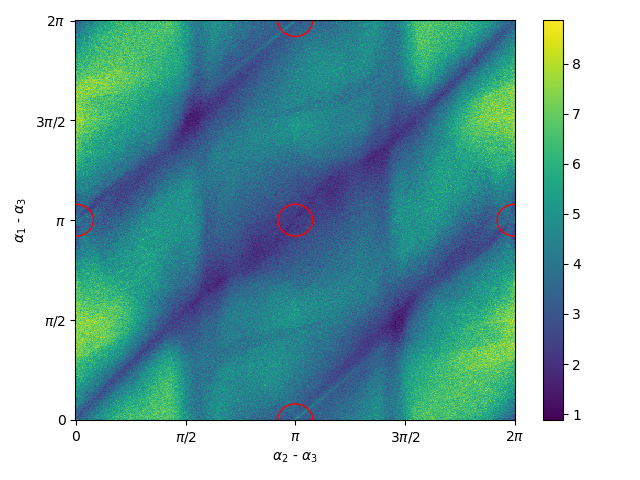
\includegraphics[width=\textwidth]{Figures/max eigen_Alpha 2 - Alpha 3-Alpha 1 - Alpha 3.png}
\end{subfigure}
\hfill
\begin{subfigure}{0.49\textwidth}
    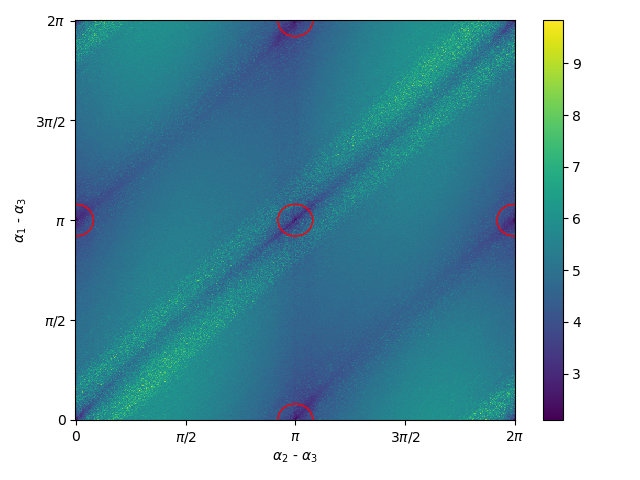
\includegraphics[width=\textwidth]{Figures/solver iterations_Alpha 2 - Alpha 3-Alpha 1 - Alpha 3.png}
\end{subfigure}
        
\caption{Mesh grids of $|\Re(\lambda_j(s))|$ (left) and solver iterations $k$ (right) with respect to the relative axial angles. $20,000,000$ random configurations were sampled. The stability equilibria points are $(0, \pi)$, $(\pi, 0)$, $(\pi, \pi)$, $(\pi, 2\pi)$, and $(2\pi, \pi)$ \cite{GilbertHendrickWebster_TRO_2016}.}
\label{fig:mesh_grids}
\end{figure*}

Snaps or bifurcations in a CTCR system occur due to built-up torsional energy, causing a sudden configuration change as the robot releases the stored tension \cite{WebsterRomanoCowan_TRO_2009}.
This snapping happens when the robot suddenly transitions from a local minimum energy state to a global minima, forcing a snap to occur \cite{WebsterRomanoCowan_TRO_2009}.
Elastic instability in a CTCR increases as the relative axial angle -- the absolute difference between the actuator's rotations -- approaches $\pi$, where instability is maximized \cite{WebsterRomanoCowan_TRO_2009, Bergeles_TRO_2015}.
After a bifurcation, the system reaches a stable equilibrium state, which typically occurs when the robot's tubes are aligned or anti-aligned \cite{GilbertHendrickWebster_TRO_2016}.
}

\bulletpoints{
    \item Topic Sentence: Discuss the experimental setup for supporting our hypothesis
    \item Static Cosserat Rod don't model dynamic energy interactions but conditioning can help us with it
    \item Equilibrium points should result in a well-conditioned system
    \item We sample 20 million configurations and generated mesh plots to visualize the conditioning wrt axial angles
}

\commentblock{
Although the static Cosserat Rod equations do not model dynamic energy interactions, they do capture the torsional energy present within the tubes.
As such, the system's elastic stability can be indirectly inferred from the ODE system's conditioning, with configurations at the equilibrium points resulting in a well-conditioned system.
To test our hypothesis, we sampled 20,000,000 random configurations and generated mesh plots of the non-linear solver's iteration count $k$ and the BVP's stiffness value $|\Re(\lambda_j(s))|$ relative to the axial angles.
These values indicate the system's conditioning, as they are influenced by the conditioning of $A$ \cite{Heath_SIAM_2018}.
}

\bulletpoints{
    \item Topic Sentence: Discuss the findings and why they support our hypothesis
    \item Areas with low stiffness overlap with equilibria
    \item Quick convergence is strongly correlated with equilibria points
    \item Coincidence with (0, 0) and (2pi, 2pi) due to default guess being correct
    \item Equilibria affects stiffness but there seems to be other stronger forces.
    \item Maybe a sentence about using the proxy planning stable paths and avoiding snapping behaviour
}

\commentblock{
As shown in Fig. ~\ref{fig:mesh_grids}, areas with low stiffness overlap with equilibrium points.
Furthermore, the non-linear solver converges the quickest around regions of equilibria, with clusters of minimal iteration counts centered exactly at the equilibrium points.
Regions surrounding points with no changes in the relative axial angles, such as $(0, 0)$ and $(2\pi, 2\pi)$, also show fast convergence due to the initial guess of zero torsional forces at the base coinciding with the correct solution.
Although elastic stability might affect stiffness, other factors seem to have a stronger influence.
This is evident from the clustering of eigenvalues at locations other than the equilibrium points.
}

\subsection{Future Work}

\bulletpoints{
    \item Topic Sentence: Discuss the jacobian A and how it needs to be investigated further
    \item Although we have jacobian A, more work needs to be done to get a reliable upper-bound.
    \item Having an upper-bound to A would give us a deeper understanding of the problem's stiffness and shed light on the elements influencing it.
    \item Also, it might helps us determine the reason of the clusters for the eigenvalues
    \item It might also explain the two-bands of abnormally large k
}

\commentblock{
Although the Jacobian matrix $A$ was introduced for the ODE system governing the BVP, an analytical upper bound for it has yet to be derived.
Such an upper bound would provide deeper insights into how the robot's parameters affect stiffness and identify which elements most significantly influence the system's conditioning.
It could also clarify the clustering behavior of the $|\Re(\lambda_j(s))|$ values and explain why they differ from solver convergence.
Furthermore, additional runtime improvements may be possible if a relationship between the optimal torsional values at the base and the eigenvalues of $A$ were to be discovered.
A thorough examination of $A$ would reveal whether such a relationship exists and how it could be exploited.
}

\bulletpoints{
    \item Topic Sentence: Discuss the proxy and how it needs to be investigated further.
    \item An in-depth investigation still needs to determine if k is a reliable indicator of stability
    \item The investigation should also examine how k could be used for planning stable paths and avoiding snapping
    \item Relationships between stiffness and the torsional forces at the base should be investigated
    \item If there is such a relation, it might provide us with a way to obtain a reliable estimate resulting in faster converging.
}

\commentblock{
Further research is necessary to determine whether the convergence count $k$ consistently serves as a reliable indicator of relative elastic stability. This investigation should explore the behavior of this numerical proxy under various scenarios, including extreme use cases, and demonstrate its practical application. The numerical proxy should also be integrated into a path planner, with the algorithm's performance evaluated in detail. If the numerical proxy proves reliable, it could be leveraged for real-time path planning and the avoidance of snapping behavior \cite{GilbertHendrickWebster_TRO_2016}.
}

%===============================================================================
% Conclusion
\section{CONCLUSIONS}

\bulletpoints{
    \item Topic Sentence: The take home message is that we were able to achieve real-time runtime while maintaining universality.
    \item Our approach is entirely numerical
    \item We achieved 120 microsecond runtime and maintained universality
    \item We also have a potential proxy
}

\commentblock{
This investigation covers explicit integration techniques, quaternion-based orientation representation, and efficient Jacobian updating schemes, resulting in significant reductions in the computational runtime of the forward kinematics of the Cosserat Rod model.
By combining the proposed optimizations, we demonstrate a reduction of up to $90\%$ in function calls with no loss in accuracy.
Our optimized kinematic model achieves an average runtime of just \SI{120}{\mu s}, making it suitable for high-frequency, real-time control of CTCR systems while also ensuring broad applicability across various architectures and systems.
Furthermore, we introduced a novel, computationally accessible proxy for elastic stability, which holds promise for detecting snapping behavior in CTCRs.
}

%\footnotetext{\url{https://github.com/ContinuumRoboticsLab/CRVisToolkit}}


%%%%%%%%%%%%%%%%%%%%%%%%%%%%%%%%%%%%%%%%%%%%%%%%%%%%%%%%%%%%%%%%%%%%%%%%%%%%%%%%

% \addtolength{\textheight}{-12cm}   % This command serves to balance the column lengths
%                                   % on the last page of the document manually. It shortens
%                                   % the textheight of the last page by a suitable amount.
%                                   % This command does not take effect until the next page
%                                   % so it should come on the page before the last. Make
%                                   % sure that you do not shorten the textheight too much.

%%%%%%%%%%%%%%%%%%%%%%%%%%%%%%%%%%%%%%%%%%%%%%%%%%%%%%%%%%%%%%%%%%%%%%%%%%%%%%%%



%%%%%%%%%%%%%%%%%%%%%%%%%%%%%%%%%%%%%%%%%%%%%%%%%%%%%%%%%%%%%%%%%%%%%%%%%%%%%%%%



%%%%%%%%%%%%%%%%%%%%%%%%%%%%%%%%%%%%%%%%%%%%%%%%%%%%%%%%%%%%%%%%%%%%%%%%%%%%%%%%
\section*{ACKNOWLEDGMENT}
The authors would like to thank Sébastien Briot and Andrea Gotelli for discussions aiding in the conceptualisation of this paper.


\addcontentsline{toc}{section}{REFERENCES}
\bibliographystyle{IEEEtran}
\bibliography{IEEEabrv, literature}

%%%%%%%%%%%%%%%%%%%%%%%%%%%%%%%%%%%%%%%%%%%%%%%%%%%%%%%%%%%%%%%%%%%%%%%%%%%%%%%%


\end{document}